\documentclass[a4paper,superscriptaddress,nofootinbib]{revtex4}

\addtolength{\oddsidemargin}{1cm}
\addtolength{\evensidemargin}{1cm}
\addtolength{\textwidth}{-2.6cm}

% Packages
\usepackage[caption=false]{subfig}  % needed for compatibility btw revtex and captions
\usepackage{dcolumn}   % needed for some tables
\usepackage{graphicx}
\usepackage{titlesec}
\usepackage{amsmath}
\usepackage{amssymb}
\usepackage{amsthm}
  \newtheorem{theorem}{Theorem}
  \newtheorem{lemma}[theorem]{Lemma}
  \newtheorem{definition}[theorem]{Definition}
\usepackage{tikz}
\usepackage[utf8]{inputenc} % for at få danske karakterer. Kræver at alle bruger en editor som understøtter utf8.

% Macros
\definecolor{mygreen}{rgb}{0,0.6,0}
\newcommand{\at}{\makeatletter @\makeatother}
\newcommand{\tmin}{t_{\min}}
\newcommand{\tmax}{t_{\max}}

\iffalse
% Style parameters
\setlength{\parskip}{0pt}
\setlength{\tabcolsep}{6pt}
\setlength{\arraycolsep}{2pt}
\titlespacing*{\section}
{0pt}{2ex}{1ex}
\titlespacing*{\subsection}
{0pt}{2ex}{1ex}
\titlespacing*{\subsubsection}
{0pt}{2ex}{1ex}
\fi

\graphicspath{{../plots/}{../images/}}


\begin{document}

\title{Supplementary Material for \\
The Curse of Shared Knowledge: Recursive Belief Reasoning in a Coordination Game with Imperfect Information}
\author{Thomas Bolander}
\affiliation{Department of Applied Mathematics and Computer Science, Technical University of Denmark, Richard Petersens Plads, building 324, DK-2800 Lyngby, Denmark}
\author{Robin Engelhardt}
\author{Thomas S. Nicolet}
\affiliation{Center for Information and Bubble Studies, Department of Communication, University of Copenhagen, Karen Blixens Plads 8, DK-2300 Copenhagen S.}

\maketitle
%\normalsize
%\onecolumngrid

% NB: Requires formatting

\iffalse
\section*{This PDF includes:}
Supplementary text \\
Figs FIG.1 to FIG.7 \\
Table 1\\
Captions for Databases \\
References for SI citations 


\clearpage
%\appendix
\fi

%{\Huge \center Supplementary Information\\}

@@@add DIS game rules. 


@@@transcripts of DIS interviews (only selected ones here, I guess)


\subsection*{MTurk Walkthrough and Screenshots}
\begin{figure} %[h]
\centering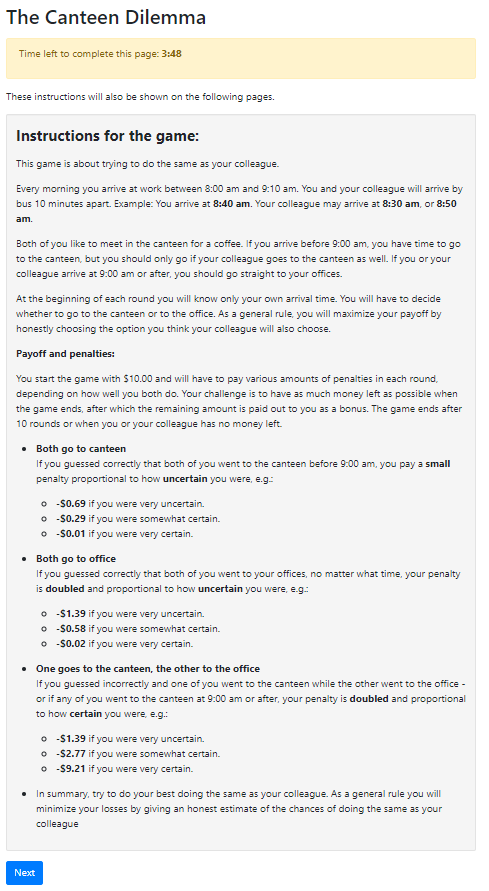
\includegraphics[width=0.8\linewidth]{screenshot_instructions}
\caption{Screenshot of instructions page.}
\label{fig:instructions}
\end{figure}
\begin{figure} %[h]
\centering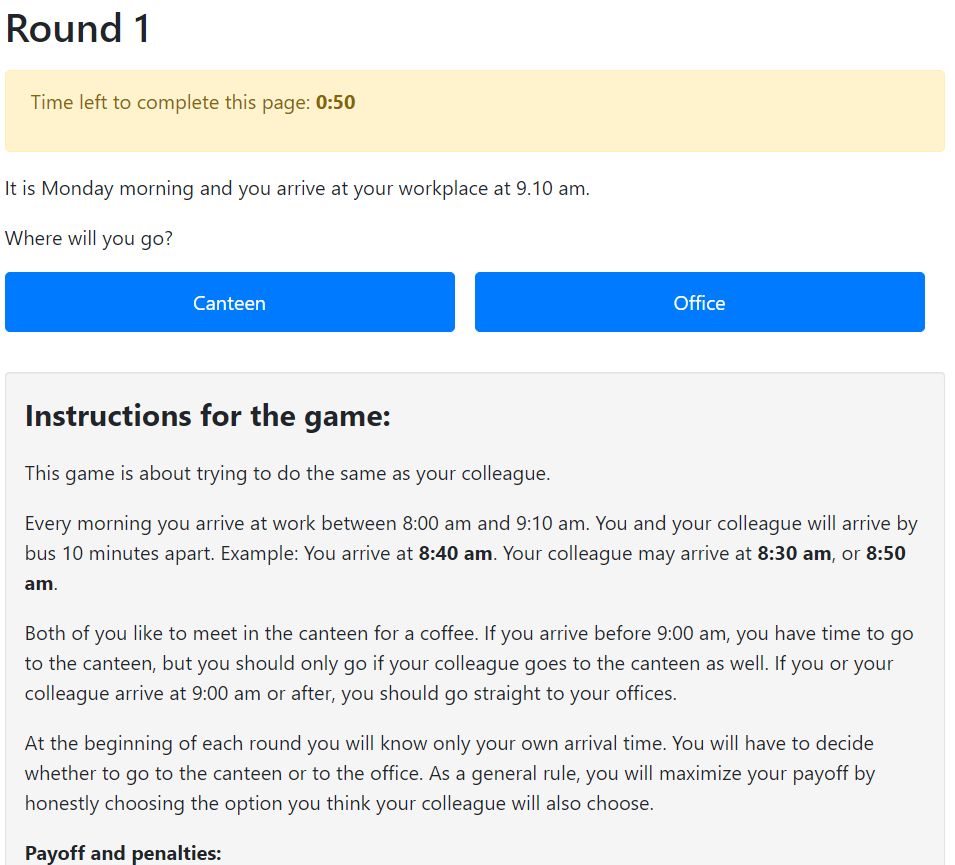
\includegraphics[width=0.8\linewidth]{screenshot_round1}
\caption{Screenshot of choice page, round 1.}
\label{fig:round1}
\end{figure}
\begin{figure} %[h]
\centering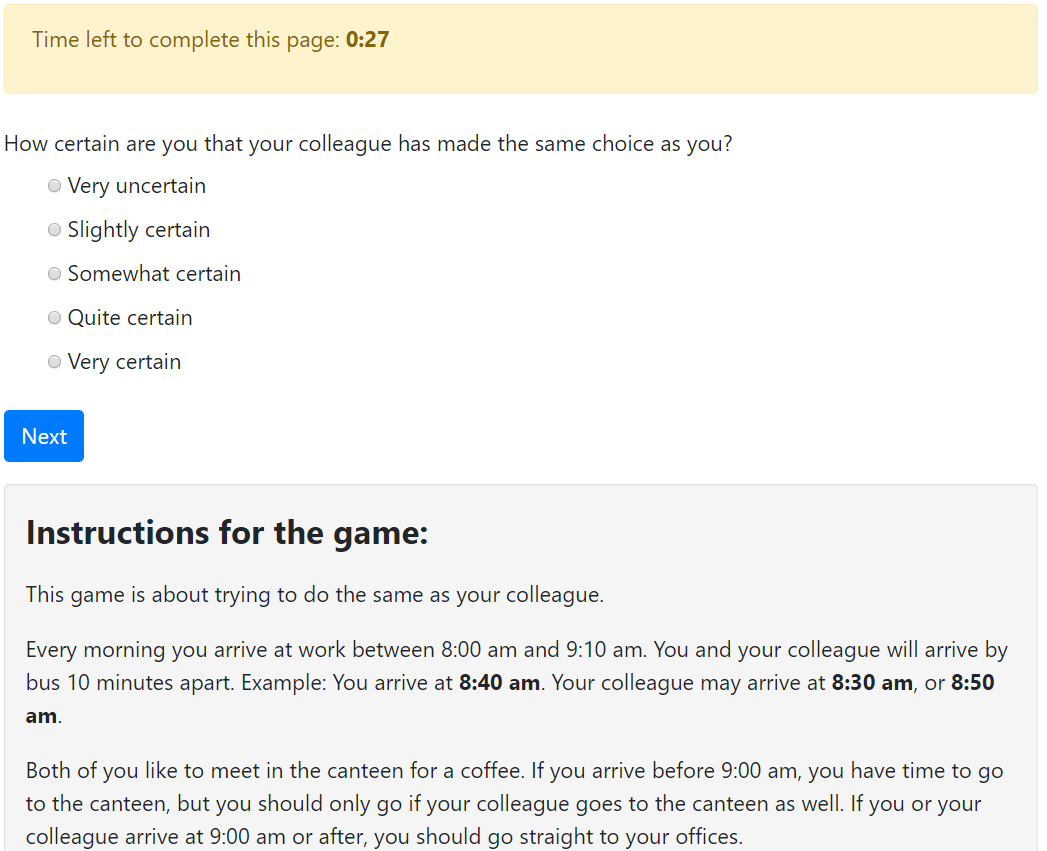
\includegraphics[width=0.8\linewidth]{screenshot_certainty}
\caption{Screenshot of page where participants had to estimate the probability that their colleague would make the same choice.}
\label{fig:certainty}
\end{figure}
\begin{figure} %[h]
\centering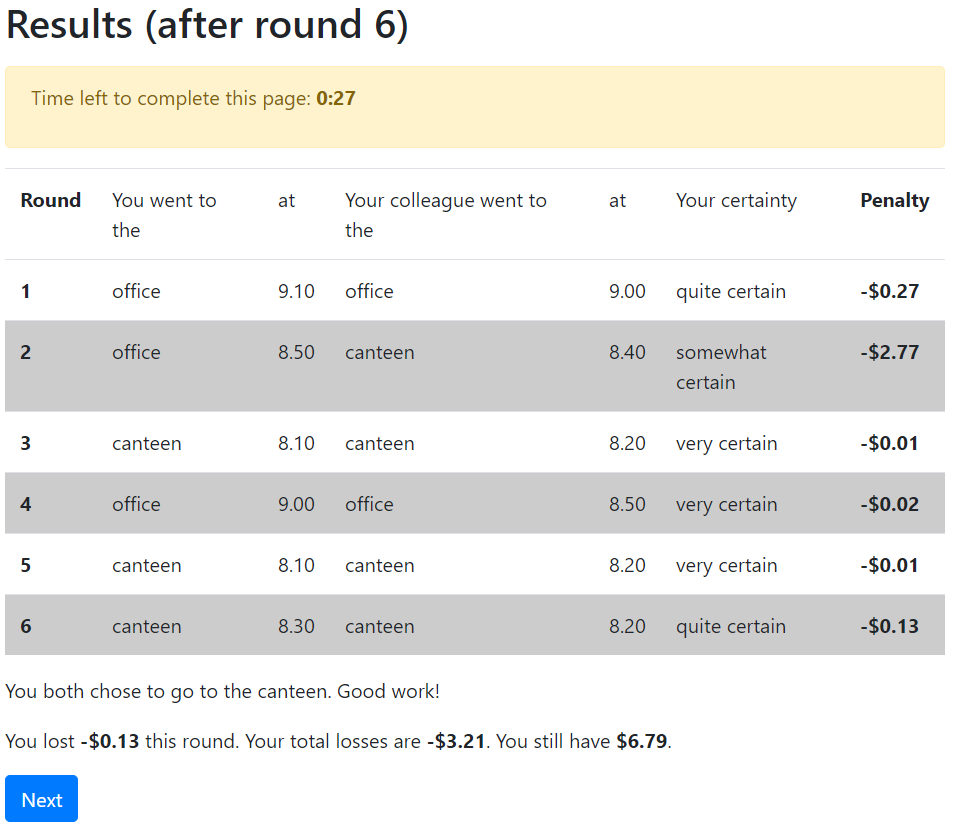
\includegraphics[width=0.7\linewidth]{screenshot_round6results}
\caption{Screenshot of results page, round 6.}
\label{fig:results6}
\end{figure}
\begin{figure} %[h]
\centering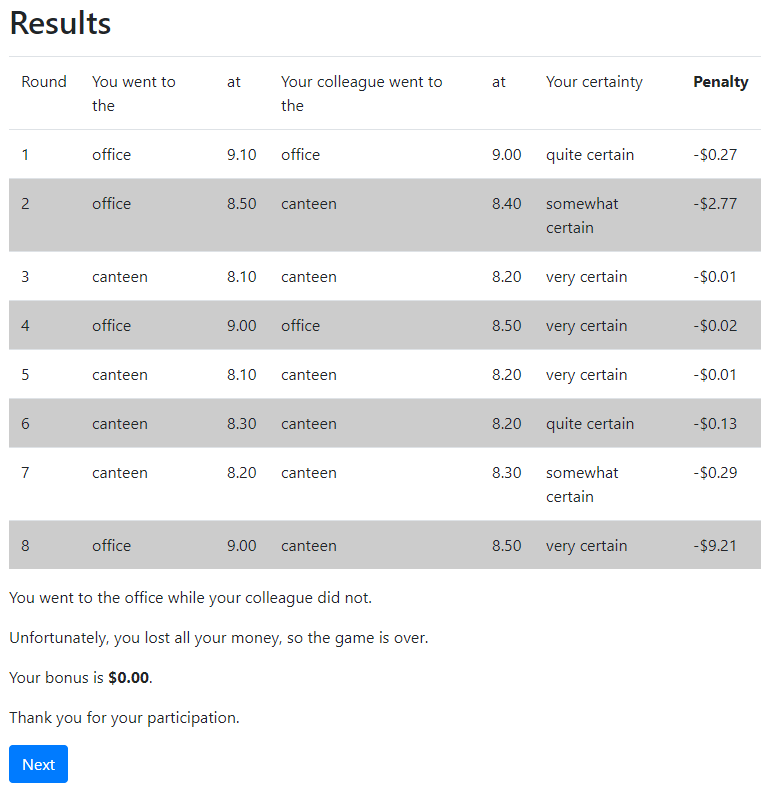
\includegraphics[width=0.7\linewidth]{screenshot_round8finished}
\caption{Screenshot after a player has lost all her bonus.}
\label{fig:round8finished}
\end{figure}
After accepting our `Human Intelligence Task' (HIT) and providing informed consent, participants from MTurk were put in a ’waiting room’ until they were paired up with another participant. After a group of two was formed, participants were directed to an initial instruction page which detailed the rules of the game with a time limit of 240 seconds, see screenshot in Fig.~\ref{fig:instructions}.
After reading the instructions, participants were directed to round 1 (of 10) where they were given their own arrival time and asked to make a decision between between going to the canteen or the office. Each round had a time limit of 61 seconds and rules from the instructions were repeated on the bottom of the page, see example screenshots for round 1 in Fig.~\ref{fig:round1}.

After making their decision (`Canteen' or `Office'), participants were asked to estimate how certain they were that the other player made the same choice as them, ranging from `very uncertain' over `slightly certain', `somewhat certain' and `quite certain' to `very certain', see Fig.~\ref{fig:certainty}.

After both players have made their choices and their certainty estimates, they are prompted to a results page showing them the results of the previous rounds, including arrival times for both players, their choices, their own certainty estimate and resulting payoff, see example screenshot after round 6 in Fig.~\ref{fig:results6}. After 30 seconds, the game would automatically proceed to the next round.

In many instances, groups were not able to play the maximal number of rounds, because one or both of the participants had lost all their bonuses. An example of such a situation is shown in Fig.~\ref{fig:round8finished}. In such cases, the game would end for both players and they were asked to answer a follow-up question: 


\begin{quote}
\indent
1. ``The game is over. Do you think it was your fault it is over, your colleagues fault, or do
you think it was because of some other reason?'' \textit{(Possible answers: `My fault', `Other's fault', `Other reason')}
\end{quote}
This question probes into participants' ability to rise above their possibly myopic understanding of the game. In addition to this question, all participants were asked three additional post-game questions about their strategy of play and their understanding of the game. The first was:
\begin{quote}
\indent
2. ``What strategy did you use while playing this game?" \textit{(open ended)}
\end{quote}
The answers to this question provided insight into the reasoning and thoughts of the participants. The next question was used to gauge the depths of recursive reasoning and reads:
\begin{quote}
\indent
3. ``Imagine you could have agreed beforehand with your colleague about a point in time where it is safe to go to the canteen. What time would that be?" \textit{(`I don't know', `There is no such time', 8:00, 8:10, 8:20, 8:30, 8:40, 8:50, 9:00, 9:10)}
\end{quote}
A final question pertaining all participant's understanding of the concept of common knowledge was the following:
\begin{quote}
\indent
4. ``Imagine you arrive at 8:10 am. Is it common knowledge between you and your colleague that it is safe to go to the canteen, that is, you both arrived before 9:00 am?''. \textit{(`Yes', `No', `Don't know')}
\end{quote}


\subsection*{DTU Experiments}
The DTU students were asked three additional post-game questions:
\begin{quote}
5. ``Did you ever go to the canteen at an arrival time later than what was safe according
to your previous answer? Why or why not?'' \textit{(open ended)}
\end{quote}
\begin{quote}
6. `Did you ever choose differently after seeing the same arrival time again at a later point
in the game? Why or why not?" \textit{(open ended)}
\end{quote}
\begin{quote}
7. `Imagine you arrived at [8:40/9:00] and you have been secretly informed that your colleague’s arrival time is 8:50. Where do you think your colleague will go?'' \textit{(`Canteen', `Office')}
\end{quote}
In the last question, half of the participants were given 8:40 as their own arrival time while the other half were given 9:00. The question concerns whether player’s own knowledge of the other’s arrival time affect their prediction of the other player’s decision. It relates to the curse of knowledge \cite{birch2007curse} since participants might attribute their own belief (that it is early enough or too late to go to the canteen) to the other player.

\subsection*{MTurk Settings}
\label{MTurksettings}
Looking at Table \ref{table:A1}, the average payout to MTurk-workers was \$4.17 (including a general participation fee of \$2) which amounts to an average of more than \$20 per hour, which is considered very generous according to MTurk guidelines and certainly above the recently estimated average of \$6 per hour when excluding un-submitted and rejected work \cite{HaraEtAl18}. Students in the DTU experiments (DTU1 and DTU2) did not receive any monetary reward, but were told to try to maximize their payoff, and awarded prizes for doing well.

\begin{table} %[h]
\centering
\begin{tabular}{lccccc}
\hline
Experiment   &   Participants &   Attrition rate &   N & Rounds & AvgPayout  (\$) \\
\hline
 MTurk 	& 714 &  0.02 &  680 & 10 & 4.36    \\
 DTU1  	& 106 &  0.13 &  80 & 30 & (prizes)   \\
 DTU2  	&   50 &  0.08 &  42 & 30 & - \\
\hline
\end{tabular}
\caption{The main experiment on Amazon Mechanical Turk (MTurk) had 714 participants of which 17 participants (2,4 \%) quit prematurely, some of them quite early in the game. These quitters were told (in the consent form) that they would receive no bonus and no participantion fee. They are excluded from the data analysis. Their ``lucky'' colleagues however, got both their bonuses and participation fee, but are likewise excluded from the data analysis. Therefore the final number of subjects, $N$, is reduced by twice the attrition rate. In the two DTU experiments with students from the Technical University of Denmark (DTU1 and DTU2) attrition rates were slightly higher, mainly due to the higher number of rounds played.}
\label{table:A1}
\end{table}

Participants quitting a study before completing it is prevalent on MTurk, and varies systemically across experimental conditions \cite{ZhouFishbach16}. In our experiments on Amazon Mechanical Turk attrition rates were $2\%$, witnessing that we had managed to design the experiment in a way that minimized drop-out rates. A combination of high payouts, a logarithmic scoring rule taking advantage of loss aversion biases, a consent form stipulating the revocation of the participation fee after dropout, and minimization of waiting times may have been the main reasons.

All participants automatically received a `qualification' when accepting a HIT. This qualification ensured that participants could not play the game again. In addition, we required that participants should have had completed at least 500 HITs, have an accepted HIT rate of 98\% or above, and should be from the United States or Canada. This ensured that we would get relatively experienced and qualified participants.

MTurk participant attention was expected to be equal to or better than undergraduate participant’s attention \cite{Rand2012}, while various forms of dishonesty (practical joking or trying to pair up with a friend) was expected to be rare, due to the high turnover rate experienced for our HITs. In addition, during the experiment, participants had easy access to our email for questions and possible bug reports. Apart from a few timeouts, participants had no comments or complaints.

\section*{Formal definitions of Private, Shared and Common Knowledge}
\label{A:definitions}
We can define the notion of common knowledge and related notions a bit more precisely as follows, following the conventions from epistemic logic (see e.g.\ Herzig and Mauffre~\cite{herzig2015share}). Given a proposition $p$ and an agent $i$, we use $K_i p$ to denote that agent $i$ knows $p$. Given a group of agents $G = \{1,\dots,m\}$, we say that $p$ is \emph{private knowledge} in $G$ if at least one of the agents know $p$, that is, if $K_i p$ is true for some $i \in G$. We use $E_G p$ to denote that everybody in $G$ knows $p$, that is, for all $i \in G$, it is true that $K_i p$. Whenever it is not necessary to be explicit about the group of agents $G$, we will just write $E p$ and say ``everybody knows $p$''. For all $n$, we then recursively define $E^n p$ to be shorthand for $E E^{n-1} p$, where $E^1 p$ is shorthand for $E p$. So for instance $E^2 p$ expresses that ``everybody knows that everybody knows that $p$'', and in general $E^n p$ means we have $n$ iterations of ``everybody knows that'' in front of $p$. We read $E^n p$ as ``everybody knows $p$ to depth/order $n$''. We also call this \emph{shared knowledge} (of $p$) to depth/order $n$, or \emph{$n$th-order shared knowledge}. When we say that $p$ is \emph{shared knowledge}, we mean that it is shared knowledge to depth $n$ for some $n \geq 1$. \emph{Common knowledge} of $p$ then means that $E^n p$ is true for all $n \in \mathbb{N}$.

In epistemic logic, the three notions---private, shared and common knowledge---are usually not considered to be mutually exclusive. So if $p$ is common knowledge, it is also automatically both shared and private, since when the conditions for $p$ being common knowledge are satisfied, also the conditions for it being shared and private are satisfied. However, in many cases, as in our paper, we want to make an exclusive distinction between the three types of knowledge. We can define $p$ to be \emph{shared knowledge only} if it is shared knowledge but not common knowledge. Thus, $p$ is shared knowledge only if for some $n$ we have $E^n p$ but not $E^{n+1} p$. Similarly, we can say that $p$ is \emph{private knowledge only} if $p$ is private but not shared knowledge. Thus, $p$ is private knowledge only if $K_i p$ holds for some, but not all, $i$. In most texts, as in ours, it is left implicit whether private and shared knowledge are interpreted inclusive or exclusive, that is, one doesn't explicitly distinguish between ``shared knowledge'' and ``shared knowledge only''. Normally it is clear from the context whether one intends the concept to be interpreted exclusively or inclusively. 

In our paper, we interpret the concepts exclusively, although we make an exception for private knowledge. When $p$ is known by all agents, we say that $p$ is both private and (first-order) shared knowledge. The exact border between private and shared knowledge vary significantly between different papers. De Freitas et al.~\cite{de2019common} consider the case $E p$ to still only be private knowledge, and for $p$ to be considered shared knowledge furthermore requires that there is at least one agent $i$ knowing $E p$ to be true (that is, requires $K_i E p$ to be true for some $i \in G$). The point of De Freitas et al.\ is that if only $E p$ is true, it is not really shared knowledge, but only private knowledge held by everyone in $G$. In our paper, we have sought a compromise between the terminology by De Freitas et al. and the standard terminology in epistemic logic, and hence we have the overlap between private and shared knowledge.

\section*{Supporting data analysis}
\begin{figure} %[htb]
\subfloat[\label{fig: logit mturk}]{%
  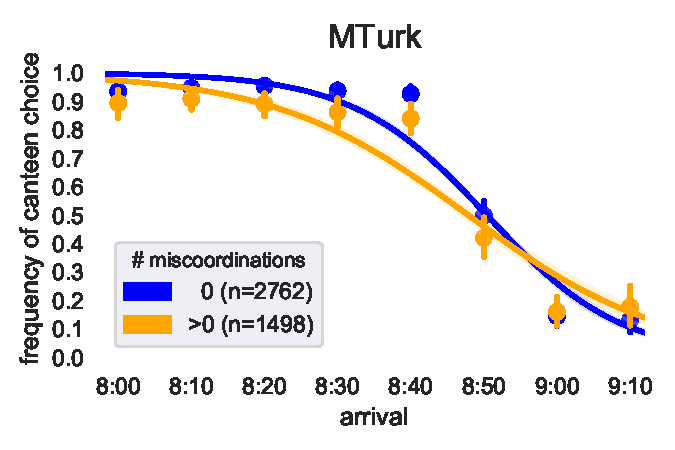
\includegraphics[width=.46\linewidth]{figS6_logit_2bins_MTurk}%
}\hfill
\subfloat[\label{fig: logit dtu}]{%
  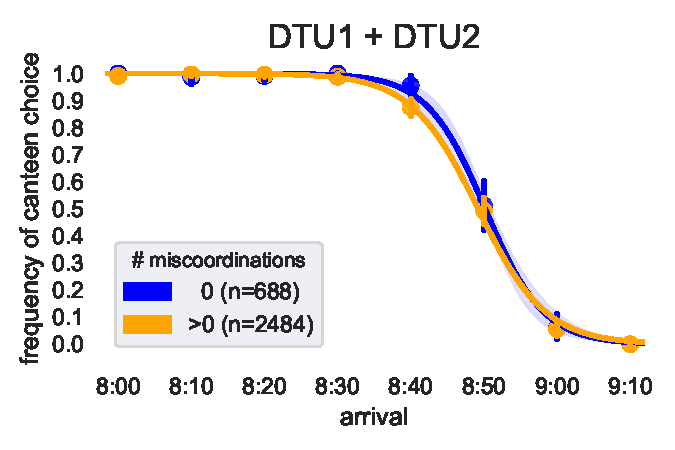
\includegraphics[width=.46\linewidth]{figS6_logit_2bins_DTU}%
}\hfill
\caption{Participant's decisions of going to the canteen as a function of their arrival time, here partitioned into those groups who previous have experienced zero (blue) or one or more (orange) miscoordinations. MTurk participants are shown one the left, DTU students on the right}\label{fig:miscoordinations}
\subfloat[\label{fig: certain mturk}]{%
  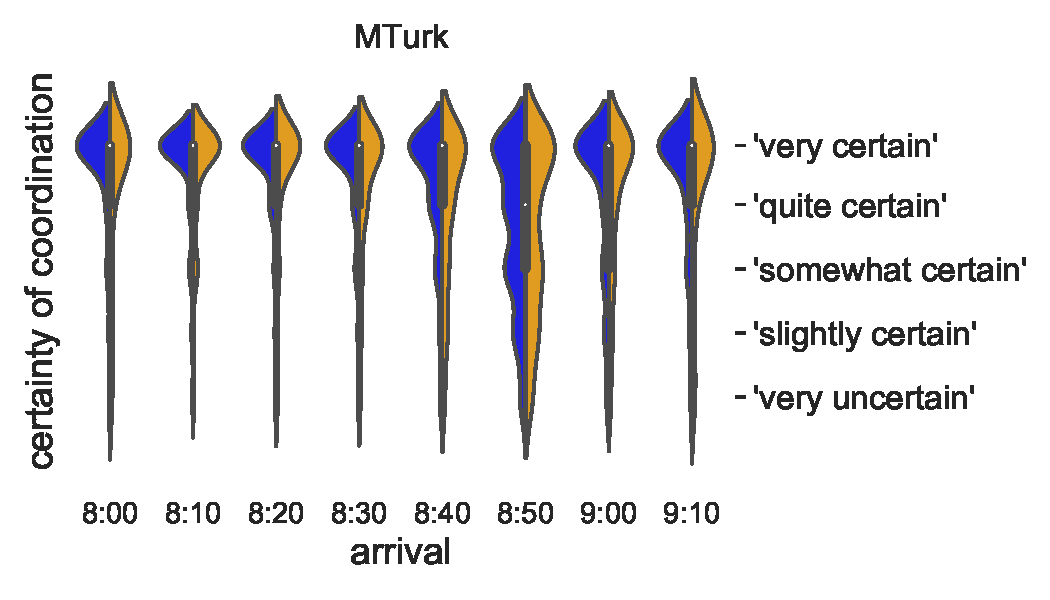
\includegraphics[width=.46\linewidth]{figS7_certainties_MTurk}%
}
\subfloat[\label{fig: certain dtu}]{%
  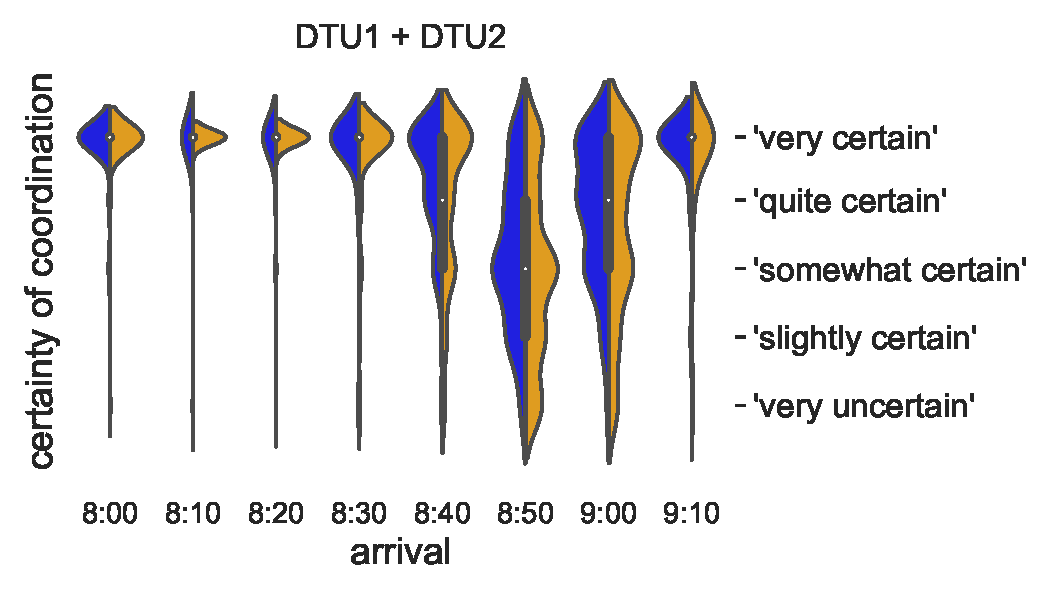
\includegraphics[width=.46\linewidth]{figS7_certainties_DTU}%
}
\caption{Participant's certainty estimates of being able to coordinate with their colleauge as a function of their arrival time, partitioned into those groups who previous have experienced zero (blue) or one or more (orange) miscoordinations. MTurk participants are shown one the left, DTU students on the right}\label{fig:certainties}
\end{figure}
When a group experiences a round of miscoordination, we expect some kind of learning to take place. `Why did my colleague choose differently than I did?' should be an obvious question a player asks herself, prompting deeper perspective-taking and possibly an understanding of the lack of common knowledge. We investigate this by partitioning decisions into those in which a participant never before has experienced a miscoodination with her colleague ($m=0$) and those in which a participant has experienced one or more miscoodinations ($m>0$). Furthermore, since the number of rounds - and hence miscoordinations - are very different for MTurk participants and DTU students, results from MTurk and DTU are shown separately, with the two DTU experiments combined. Results for the choices in Fig.~\ref{fig:miscoordinations} show significant differences between MTurk-groups having miscoordinated or not, while for DTU students those differences are not significant. Looking into the corresponding certainty estimates, as shown in Fig.~\ref{fig:certainties}, we see a similar pattern as before: Much steeper profiles among DTU students, but also much lower certainty estimates around critical arrival times. 

\iffalse
\section*{Datasets}
MTurk\_anonymous.xlsx, DTU1\_anonymous.xlsx, and DTU2\_anonymous.xlsx: Anonymized data set of all Mechanical Turk experiments. Parameters: session = name of experiment; code = anonymized participant id; group = group number in session; id\_in\_group = player id in group; round = round number; arrival = arrival time; choice = choice made by participant; certainty = certainty estimate by participant; bonus = penalty in dollars; strategy = free text question after game has ended; simple = answers to question 4, cutoff = answers to question 3; fault = answers to question 1; payoff = money left after game has finished.
\fi

\begin{thebibliography}{71}\small
\expandafter\ifx\csname natexlab\endcsname\relax\def\natexlab#1{#1}\fi
\providecommand{\bibinfo}[2]{#2}
\ifx\xfnm\relax \def\xfnm[#1]{\unskip,\space#1}\fi

\bibitem[{Birch and Bloom(2007)}]{birch2007curse}
\bibinfo{author}{S.~A. Birch}, \bibinfo{author}{P.~Bloom},
\newblock \bibinfo{title}{The curse of knowledge in reasoning about false
  beliefs},
\newblock \bibinfo{journal}{Psychological Science} \bibinfo{volume}{18}
  (\bibinfo{year}{2007}) \bibinfo{pages}{382--386}.

\bibitem[{Hara et al. (2018)}]{HaraEtAl18}
\bibinfo{author}{K. Hara}, \bibinfo{author}{et al.},
\newblock \bibinfo{title}{A data-driven analysis of workers' earnings on amazon
  mechanical turk},
\newblock \bibinfo{journal}{Proc. of the 2018 Conference on Human Factors in
  Computing Systems ACM}
  (\bibinfo{year}{2018}) \bibinfo{pages}{449}.

\bibitem[{Zhou and Fishbach(2016)}]{ZhouFishbach16}
\bibinfo{author}{H. Zhou}, \bibinfo{author}{A. Fishbach},
\newblock \bibinfo{title}{The pitfall of experimenting on the web: How
  unattended selective attrition leads to surprising (yet false) research
  conclusions},
\newblock \bibinfo{journal}{Journal of Personality and Social Psychology} \bibinfo{volume}{111}
  (\bibinfo{year}{2016}) \bibinfo{pages}{493--504}.

\bibitem[{Rand (2012)}]{Rand2012}
\bibinfo{author}{D. G. Rand}, \bibinfo{author}{P.~Bloom},
\newblock \bibinfo{title}{The promise of {M}echanical {T}urk: how online labor markets can
  help theorists run behavioral experiments},
\newblock \bibinfo{journal}{Journal of Theoretical Biology} \bibinfo{volume}{299}
  (\bibinfo{year}{2012}) \bibinfo{pages}{172--9}.

\bibitem[{Herzig and Maffre (2015)}]{herzig2015share}
\bibinfo{author}{A. Herzig}, \bibinfo{author}{F. Maffre},
\newblock \bibinfo{title}{How to share knowledge by gossiping},
\newblock \bibinfo{journal}{Springer}
  (\bibinfo{year}{2015}) \bibinfo{pages}{249--263}.

\bibitem[{De~Freitas et~al.(2019)De~Freitas, Thomas, DeScioli, and
  Pinker}]{de2019common}
\bibinfo{author}{J.~De~Freitas}, \bibinfo{author}{K. A.~Thomas},
  \bibinfo{author}{P.~DeScioli}, \bibinfo{author}{S.~Pinker},
\newblock \bibinfo{title}{Common knowledge, coordination, and strategic
  mentalizing in human social life},
\newblock \bibinfo{journal}{Proceedings of the National Academy of Sciences}
  \bibinfo{volume}{116} (\bibinfo{year}{2019}) \bibinfo{pages}{13751--13758}.
\end{thebibliography}
\end{document}